\newcommand{\textretrieval}{textretrieval-001}

\newcommand{\sustain}{sustain-001}

\newcommand{\UIUC}{UIUC}

\section{Experiment Results}
As an analysis tool, the TL-HMM model provides with us the following two
patterns to characterize student behavior:
\begin{enumerate*}[label=(\arabic*)]
  \item the latent state representations, and
  \item the latent state transitions.
\end{enumerate*}
Thus to evaluate the proposed model, we conduct experiments to
qualitatively analyze both types of patterns discovered from empirical MOOC
log data.

Specifically, we looked at the MOOC logs associated with the \textretrieval{}
Coursera MOOC offered by \UIUC{} and extracted a dataset consisting of
18,941 students who produced 85,240 sequences with an average length of
7.31. We used the following ten actions as our action set $\mathbf{A}$:
\begin{enumerate*}[label=(\arabic*)]
  \item quiz start,
  \item quiz submit,
  \item wiki (course material),
  \item forum list (view the list of all forums),
  \item forum thread list (view the list of all threads in a specific
    forum),
  \item forum thread view (view the list of posts within a specific
    thread),
  \item forum search (a search query issued against the forum),
  \item forum post thread (a new thread was posted),
  \item forum post reply (a new post was created within an existing
    thread), and
  \item view lecture (defined as either streaming or downloading a lecture
    video).
\end{enumerate*}

\subsection{Latent State Representations}
To visualize these Markov models that represent our latent states, we plot
them as a directed graph where we set the size of a node to be proportional
to its probability of being visited during a random walk.  We let the
thickness of a directed edge $(u, v)$ reflect the probability of taking
that edge given that a random walk is currently at note $u$ (as indicated
by the transition matrix)\footnote{We do not plot the transition
probabilities directly within the figure to ease readability; we instead
will mention relevant transition probabilities in the text as we discuss
the plots. The plots were created using python-igraph:
\url{http://igraph.org/python/}.}.

\begin{figure*}
  \centering
  \begin{subfigure}[t]{0.24\textwidth}
    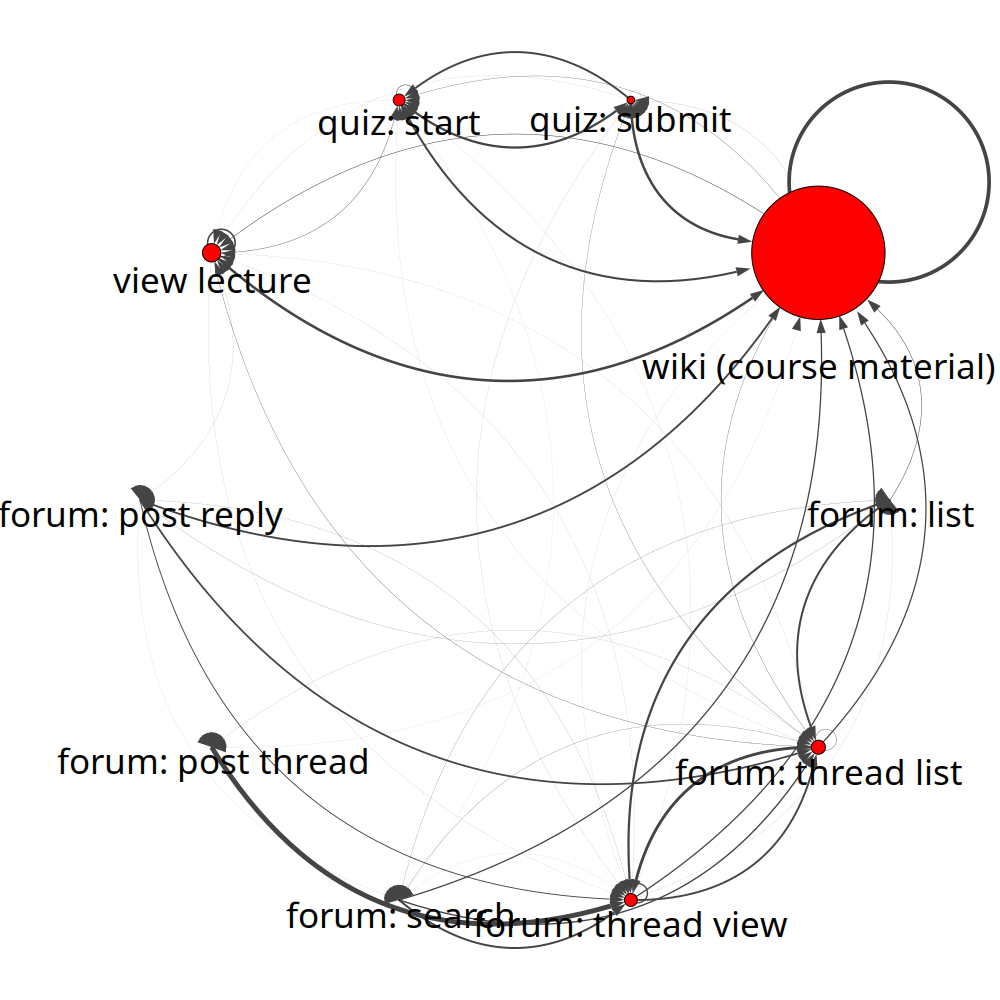
\includegraphics[width=\textwidth]{../figures/text-4state/state0.png}
    \caption{\label{fig:state0}State 0}
  \end{subfigure}
  \begin{subfigure}[t]{0.24\textwidth}
    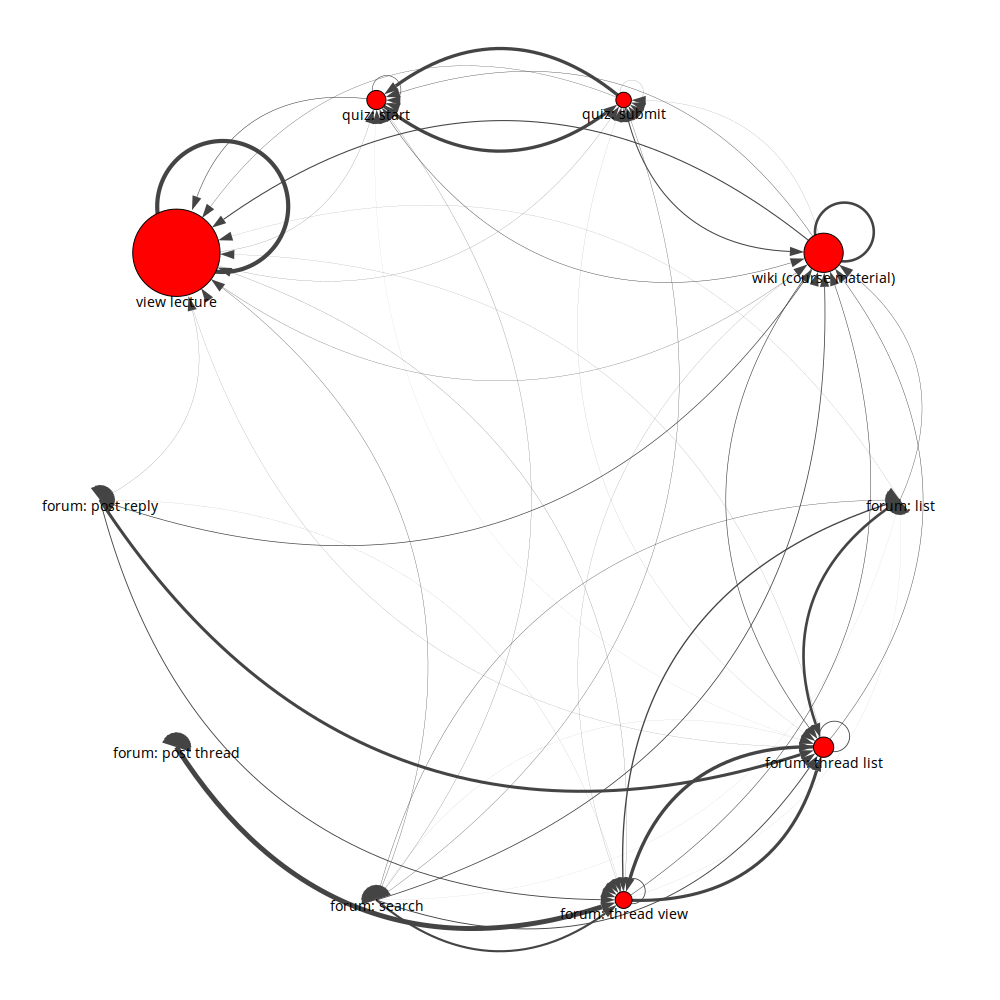
\includegraphics[width=\textwidth]{../figures/text-4state/state1.png}
    \caption{\label{fig:state1}State 1}
  \end{subfigure}
  \begin{subfigure}[t]{0.24\textwidth}
    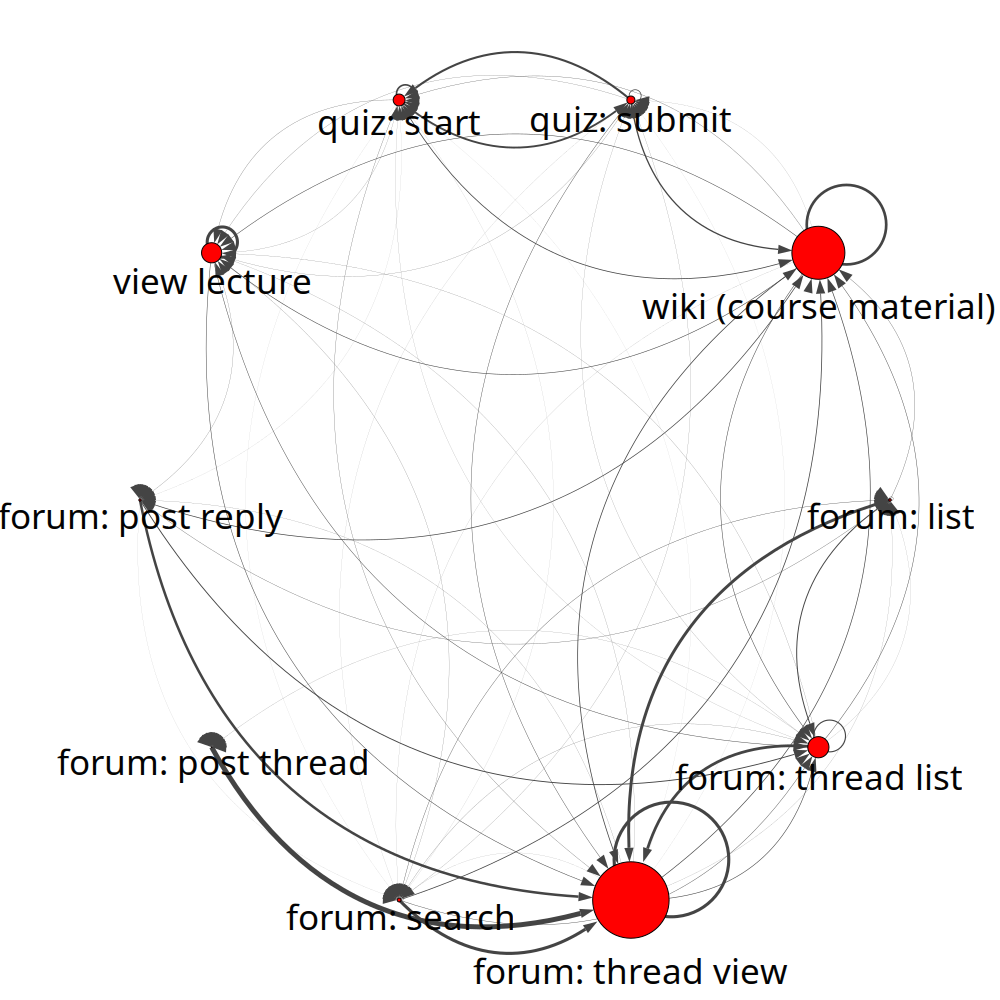
\includegraphics[width=\textwidth]{../figures/text-4state/state2.png}
    \caption{\label{fig:state2}State 2}
  \end{subfigure}
  \begin{subfigure}[t]{0.24\textwidth}
    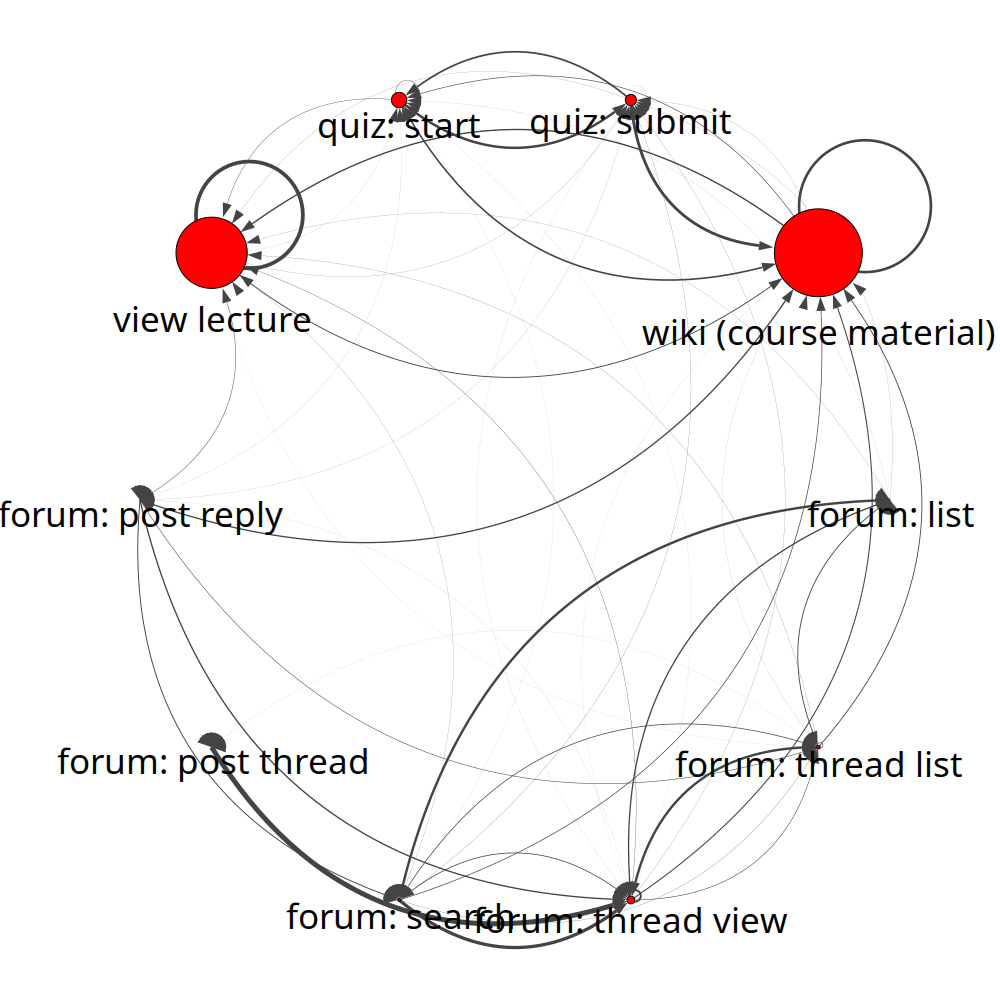
\includegraphics[width=\textwidth]{../figures/text-4state/state3.png}
    \caption{\label{fig:state3}State 3}
  \end{subfigure}
  \caption{Example states learned by a 4-state TL-HMM.}
  \label{fig:states}
\end{figure*}

Figure~\ref{fig:states} shows the latent state representations learned by
fitting a 4-state TL-HMM to the \textretrieval{} sequence dataset. Our
interpretations of the states is as follows:
\begin{enumerate*}[label=(\alph*)]
  \item \textbf{state 0} likely captures all sequences where a student
    logged in to the platform and did nothing else (likely just checking
    for updates);
  \item \textbf{state 1} seems to capture a more engaged browsing session,
    where there is non-negligible probability associated with different
    activities such as quiz taking and forum browsing and, importantly,
    these activities have high probability symmetric edges (so students are
    taking quizzes one after the other, or viewing forum threads in
    succession);
  \item \textbf{state 2} captures a ``forum browsing'' state, with most
    weight being placed on consecutive thread views; and
  \item \textbf{state 3} seems to capture a more passive student, with
    negligible probability mass associated with forum activity (with low
    symmetry in the edges). The link between ``quiz submit'' and ``quiz
    start'' (indicating quiz repetition) is also significantly lower than
    state 1.
\end{enumerate*}

\subsection{Transitions Between Latent States}
A unique property of our model is its ability to capture transitions
between the \emph{behavior patterns themselves} that are captured by the
latent states. In Figure~\ref{fig:trans-avg} we show the latent state
transition diagram for a 4-state TL-HMM fit on \textretrieval{}. We can
immediately observe two things: \begin{enumerate*}[label=(\arabic*)]
  \item each latent state has a very high ``staying'' probability, and
  \item the prevalence of each latent state matches our intuition.
\end{enumerate*}
In particular, we can see that the forum browsing state (state 2) has
relatively lower probability than the other states as we might expect. It
also makes sense that state 0 (low activity) has rather high probability.
If we look at state 1 and state 3, their relative probabilities match our
intuition as well: there should be more students exhibiting more passive
behaviors (state 3) than very active behaviors (state 1).

\begin{figure*}
  \vspace{12pt}
  \centering
  \begin{subfigure}[t]{0.25\textwidth}
    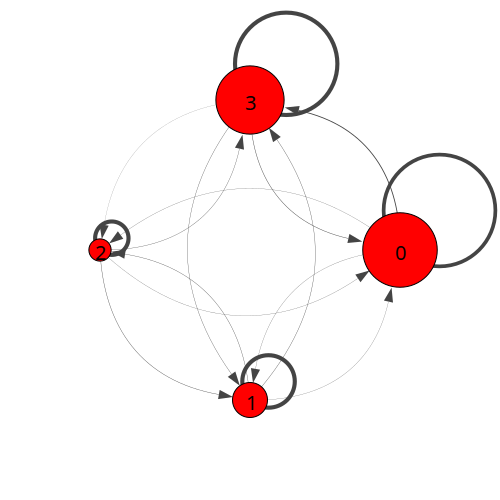
\includegraphics[width=\textwidth,trim={0 3cm 0 2cm}]{../figures/trans-comp/trans-avg.png}
    \caption{\label{fig:trans-avg}}
  \end{subfigure}%
  \begin{subfigure}[t]{0.25\textwidth}
    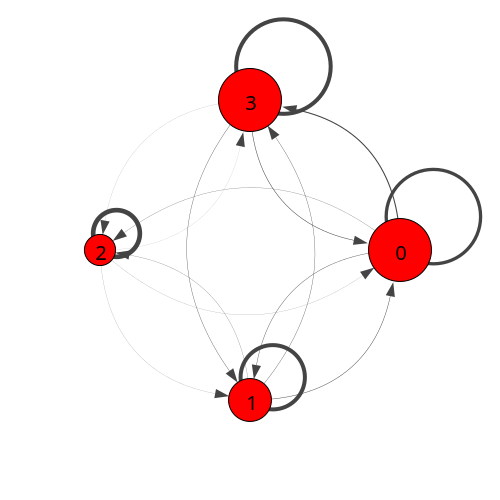
\includegraphics[width=\textwidth,trim={0, 3cm 0 2cm}]{../figures/trans-comp/trans-perfect.png}
    \caption{\label{fig:trans-perfect}}
  \end{subfigure}%
  \begin{subfigure}[t]{0.25\textwidth}
    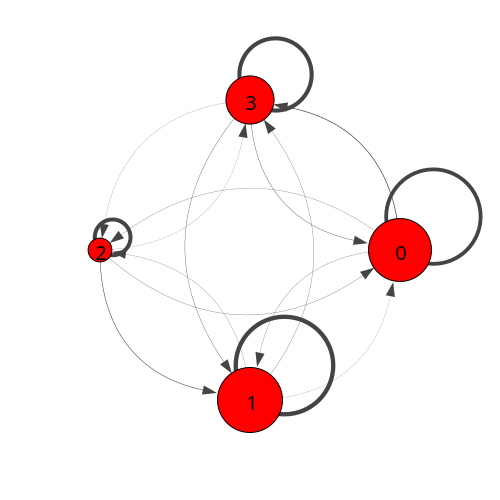
\includegraphics[width=\textwidth,trim={0, 3cm 0 2cm}]{../figures/trans-comp/trans-low.png}
    \caption{\label{fig:trans-low}}
  \end{subfigure}
  \caption{The latent state transition diagrams for a 4-state TL-HMM fit to
  \protect\textretrieval{} for all students (a) compared to only ``perfect''
  students (b) and only ``low'' students (c).}
  \label{fig:trans-comp}
\end{figure*}

Thus, we might expect to see students that perform well in the course
preferring states 1 and 2 over states 0 and 3. To verify this, we took the
model we learned on the full training data and retrofit it to training data
consisting only of sequences produced by students in \textretrieval{} that
had perfect marks. To prevent the latent state meanings from drifting, we
forced the model parameters associated with their Markov model
representations to be fixed, in effect only learning initial and transition
probabilities for the top layer of our TL-HMM.\ We show the updated latent
state transition diagram in Figure~\ref{fig:trans-perfect}. We can clearly
see that the probability of state 2 has increased dramatically, consistent
with previous observations of the positive correlation between forum
activity and grades~\cite{Huang:2014:LAS}, while the probability of states
0 and 3 has decreased. State 1 had its probability increase very slightly.

In Figure~\ref{fig:trans-low} we plot the latent state transition diagram
for a second group of ``low'' students. These students were selected so
that they attempted all required quizzes in the course, but such that their
average quiz score was $\leq 70\%$. Here, we see that \emph{state 1} has a
large increase in size, where we might have expected state 3 to grow
instead.  However, there is an alternative explanation for this phenomenon.
Since state 1 seems to indicate a highly engaged student, it is a perfectly
reasonable explanation for the ``low'' student group as they are going to
be working hard to try to fill in the gaps in their knowledge. By contrast,
the ``perfect'' student group likely has many members who can take the quiz
more passively and get perfect marks, perhaps because they already know
much of the material being presented, or are just naturally strong and do
not require much background review to perform well. This also explains why
state 1 did not increase in size for the ``perfect'' group like we were
anticipating. \citet{Kizilcec:2017:CandE} observe similar phenomena with
the courses they studied where they find that certificate earning is
negatively correlated with help seeking behavior. Our model enables
data-driven discovery of potentially counter-intuitive insights like this.

%\begin{table}
%  \centering
%  \begin{tabular}{r|rrrrr}
%    \textbf{Group} & \textbf{State 0} & \textbf{State
%  1}\textsuperscript\textdagger &
%    \textbf{State 2}\textsuperscript\textdagger & \textbf{State 3} & \textbf{State 2
%    $\rightarrow$ 2}\textsuperscript\textdagger\\\hline
%    \textbf{Perfect} & 975.3  & 1001.5 & 999.0  & 1056.5 & 939.6\\
%    \textbf{Low}     & 1024.9 & 816.4  & 1230.5 & 1161.2 & 1187.4\\
%  \end{tabular}
%  \caption{Average rank for ``perfect'' and ``low'' student groups in the
%  ranked lists associated with the four latent states found by a TL-HMM.
%  $\dagger$ indicates statistically significant different mean ranks at $p
%  < 0.01$ according to an unpaired $t$-test.}
%  \label{table:mean-rank}
%\end{table}
%
%To quantify this finding, we perform the following experiment. First, we
%select all students from \textretrieval{} who completed all of the quizzes
%$\mathbf{L}_q \subset \mathbf{L}$. This gives us 1,985 students along with
%their average quiz score. We then create a ranked list of the students in
%$\mathbf{L}_q$ by sorting them by their ``preference'' for a specific
%latent state
%\begin{equation}
%  p_\ell(i) = \frac{\sum_{t=1}^T \gamma_t^{(\mathbf{o}_\ell)}(i)}
%  {\sum_{j=1}^{K} \sum_{t=1}^T \gamma_t^{(\mathbf{o}_\ell)}(j)}
%\end{equation}
%where $\mathbf{o}_\ell$ is the list of action sequences for student $\ell$
%and $\gamma$ is defined as before and computed using the Baum-Welch
%algorithm. We can now compare the average rank in this list for both
%the ``perfect'' student group and the ``low'' student group: a useful state
%for distinguishing the two groups should result in a ranked list with
%statistically significant differences in average rank between the two
%groups. Our results are summarized in Table~\ref{table:mean-rank}. Indeed,
%we discover that states 1 and 2 are correlated with the ``perfect'' or
%``low'' groups: state 1 ranks students in the ``low'' group significantly higher
%than those in the ``perfect'' group, and state 2 does the opposite and
%prefers students in the ``perfect'' group to those in the ``low'' group.
%
%Returning to Figure~\ref{fig:trans-comp}, we an also see a difference in
%the transitions between the latent states. In particular, look at the
%transitions in Figure~\ref{fig:trans-perfect} and
%Figure~\ref{fig:trans-low} that leave state 2. In the ``perfect'' group,
%nearly all of this probability mass is allocated for the self-loop ($p
%\approx 0.93$). In the ``low'' group, this self loop is less strong ($p
%\approx 0.80$; most easily seen by noting that the edges leaving state 2
%are darker than for the ``perfect'' group). We can perform a similar
%experiment to above by producing a ranked list of students $\ell \in
%\mathbf{L}_q$ by their staying probability for state 2 (that is, given that
%a student $\ell$ is already in state 2, how likely are they to remain there
%in the next action sequence?). This can be computed as
%\begin{equation}
%  p_\ell(2, 2) = \frac{\sum_{t=1}^{T-1} \xi_t^{(\mathbf{o}_\ell)}(2,2)}
%  {\sum_{i=1}^K \sum_{t=1}^{T-1} \xi_t^{(\mathbf{o}_\ell)}(2,i)}
%\end{equation}
%where $\xi$ is defined as before and computed using the Baum-Welch
%algorithm. The last column of Table~\ref{table:mean-rank} indicates that
%this transition feature also correlates with the achievement group and
%results in significant differences in mean rank.
